% if tikzpicture not working: https://tex.stackexchange.com/a/541385

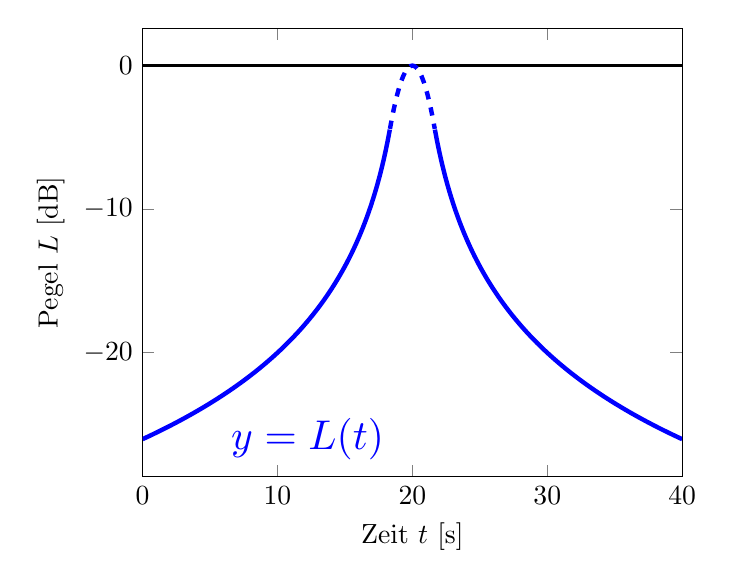
\begin{tikzpicture}
    [
        % CAUTION: in function={...} are no blank lines allowed
        declare function=
            {
                links(\x) = -20 * log10(-\x);
                inter(\x) = -1.5975 * \x*\x;
                rechts(\x) = -20 * log10(\x);
                func_l(\x) = (\x < -\d) * (links(\x));
                func_r(\x) = (\x > \d) * (rechts(\x));
                top(\x) = 0;
                dashed(\x) = and(\x >= -\d, \x <= \d) * (inter(\x));
            },
    ]

    \def\d{1.6612089648975}

    \def\xydomain{20}


    \begin{axis}
        [
            xlabel={Zeit $t$ [s]},
            ylabel={Pegel $L$ [dB]},
            xmin=0,
            xmax=2*\xydomain,
        ]
        \addplot
        [
            color=blue,
            ultra thick,
            domain=0:\xydomain-\d-0.01,
            samples=120,
        ]
        {
            func_l(x-\xydomain)
        }
        node [pos=0.2, below right, scale=1.5] {$y=L(t)$}
        ;
        \addplot
        [
            color=blue,
            ultra thick,
            domain=\xydomain+\d+0.01:2*\xydomain,
            samples=120,
        ]
        {
            func_r(x-\xydomain)
        }
        ;
        \addplot
        [
            color=black,
            thick,
            domain=0:2*\xydomain,
        ]
        {
            0
        }
        ;
        \addplot
        [
            color=blue,
            ultra thick, dashed,
            domain=-\d+\xydomain:\d+\xydomain,
        ]
        {
            dashed(x-\xydomain)
        }
        ;
    \end{axis}
\end{tikzpicture}